\documentclass[english]{article}

%% Packages pull in extra commands:
%% http://en.wikibooks.org/wiki/LaTeX/Packages
\usepackage[latin9]{inputenc}
\usepackage[letterpaper]{geometry}
\usepackage{pgfplots}
\usepackage{graphicx}
\graphicspath{ {imgs/} }
\geometry{verbose,tmargin=1in,bmargin=1in,lmargin=1in,rmargin=1in}

\title{CIS 520 Project Final Report: Twitter Gender Classification}
\author{Woodpecker (Xiang Deng, Yiren Lu, Dongni Wang)}
\date{Fall 2015}

\begin{document}
\maketitle
\section{Project Overview}
\indent \indent For the final project, we developed a system for twitter users\'s gender prediction (male/female) from the language of their tweets and their profile images. We were given a training set of 4998 labeled training samples, each has 5000 word features, 7 pre-extracted image features and 30000 raw RGB image pixel features.The time constraint for the final model(s) initialization and prediction is 3 minutes and 10 minutes, respectively, for the 5,000 test samples. Also, The submission size is limited to 50 Mb in the final checkpoint/ competition. Our submitted model for the final competition achieved an accuracy of 91.04\% on the validation set, ranked $6^{th}$ in a total of 50 2-3 people teams. \par
In our full system, we used seven classifiers on different feature sets and combined them using the stacking method.
The seven classifier are: a logistic regression model on words features, an ensemble model consists of 300 decision stump trees using LogitBoost on selected words and image features, a SVM model with intersection kernel on selected words and image features, a SVM model with intersection kernel on selected and normalized words and image features, an ANN model with 2 hidden layers each with 100 and 50 nodes, a SVM model with RBF kernel on PCA-ed HOG features on face-detected images, and a SVM model with RBF kernel on PCA-ed LBP features on face-detected images. For the stacking method, we took the raw outputs (probabilities) from the seven basic models mentioned above trained with 80\% of training samples and trained a logistic regression model using the other 20\% of training sample. Our final full model achieved an overall accuracy of 92.42\% on testing set. \par
In order to meet the time and space constraint for the competition, we dropped the SVM model on PCA-ed LBP features and replaced the SVM model on PCA-ed HOG features with one bagging of logistic regression classifiers on raw HOG features. \par
In the following sections, we present the cross-validation accuracies of each method we tried and discuss the rationale of our final model. We also provide some interesting visualization such as the most predictive words and eigenfaces.. 


\begin{figure}[h!]
\begin{center}
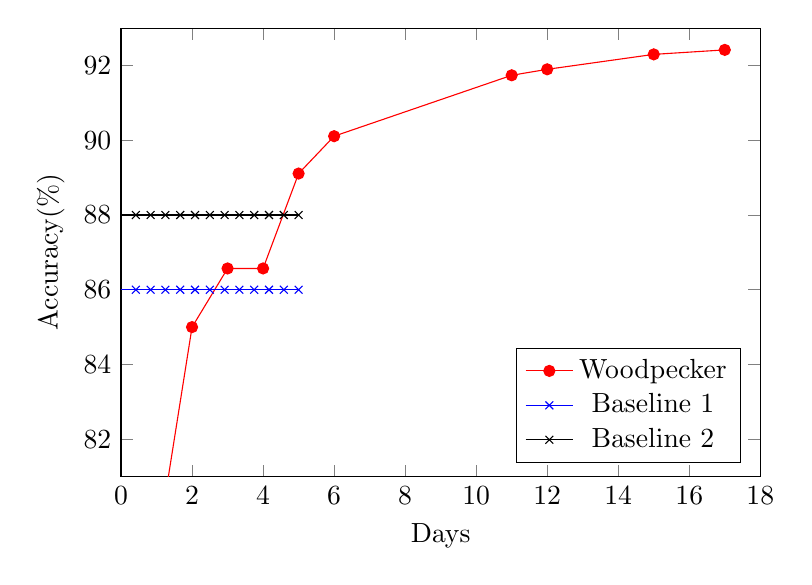
\begin{tikzpicture}
  \begin{axis}[
  		width=0.8\textwidth,
      	height=0.6\textwidth,
		xlabel={Days},
		ylabel= Accuracy(\%),
      	xmin= 0,
      	xmax= 18,
      	ymin=81,
      	ymax=93,
      	legend pos=south east],
	\addplot[color=red,mark=*] coordinates {
		(1,79)
		(2,85)
		(3,86.57)
		(4,86.57)
		(5,89.11)
		(6,90.11)
		(11,91.74)
		(12,91.9)		
		(15,92.3)
		(17,92.42)
	};
	\addplot[color=blue,mark=x]{86};
	\addplot[mark=x]{88};

\legend{Woodpecker,Baseline 1, Baseline 2}
\end{axis}
\end{tikzpicture}
\caption{The progress plot for Woodpecker}
\label{ProcessPlot}
\end{center}
\end{figure}



\section{Methods}
In this section, we report the results of multiple methods we tried for feature extraction, dimension reduction, and classification. 

\subsection{Data preprocessing}

\subsection{Feature Selection}
To extract features from the raw word and image features, we experimented with multiple feature selection methods, including Information Gain, BNS
\subsection{Dimension Reduction}
\subsection{Classification}




\section{Experiment Analysis}
In this section, we analyze the results of our experiments of multiple methods for feature extraction, dimension reduction, and classification. 
\subsection{Feature Selection/Extraction}

\subsection{Dimension Reduction}
\subsection{Classification}

\section{Discussion}
Working on this gender-classification project gave our team a chance reflected on what we have learned in class. Here is a short summary of things that have surprise us (or have taught us a lesson) 
\begin{itemize}
\item With different feature sets (especially they have various ranges and dimensions), feature selection and normalization have played an important role in improving the performances of our model. 
\item Last but not least, be careful with required formats..
\end{itemize} 

\end{document}